% =============================================================================
%  Chapitre 2 — Problématique : de l'allocation d'actifs à ses quatre échecs
%
%  Chapitre volontairement accessible : il ne suppose aucune connaissance
%  préalable en finance. Toute notion est définie à son premier emploi, dans
%  un encadré « Définition ». Les formules ne sont introduites qu'après
%  l'explication en langage courant, jamais avant.
% =============================================================================

\chapter{Problématique : de l'allocation d'actifs à ses quatre échecs}
\label{chap:problematique}

\section*{Ce que ce chapitre explique}
\addcontentsline{toc}{section}{Ce que ce chapitre explique}

Ce chapitre pose le problème que le projet cherche à résoudre. Il est écrit pour
être lu sans connaissance préalable de la finance de marché : chaque notion est
définie au moment où elle apparaît, et chaque formule est précédée de la phrase
qui dit ce qu'elle signifie.

Le fil est le suivant. Nous partons d'une question simple — comment répartir une
somme d'argent entre plusieurs placements ? — et nous montrons que la réponse
classique, formulée par Harry Markowitz en 1952 et encore enseignée aujourd'hui,
repose sur quatre hypothèses qui ne tiennent pas en pratique. Ces quatre échecs,
notés \textbf{P1} à \textbf{P4}, structurent l'intégralité du travail présenté
dans ce rapport : chaque composant développé y répond explicitement.

% =============================================================================
\section{Le problème, en une phrase}
% =============================================================================

Une banque, une compagnie d'assurance ou un particulier dispose d'une somme
d'argent et doit la répartir entre plusieurs placements. Combien mettre sur
chacun ?

La question paraît anodine. Elle ne l'est pas : c'est l'une des décisions les
plus lourdes de conséquence en gestion financière, parce qu'elle détermine à la
fois ce que l'on peut espérer gagner et ce que l'on risque de perdre. Et elle
n'a pas de réponse évidente, parce que les deux objectifs — gagner davantage et
risquer moins — s'opposent presque toujours.

L'objet de ce projet est de construire un système capable de proposer
automatiquement une telle répartition, à partir de données de marché, et de
mesurer honnêtement si ce système fait mieux que les méthodes classiques.

% =============================================================================
\section{Un portefeuille, un rendement, un risque}
% =============================================================================

\subsection{Le vocabulaire minimal}

Un \emph{actif} est un objet dans lequel on peut placer de l'argent : une action
d'entreprise, une obligation d'État, un fonds indiciel. Un \emph{portefeuille}
est simplement une répartition de capital entre plusieurs actifs : par exemple
40~\% sur l'un, 35~\% sur un deuxième, 25~\% sur un troisième. Ces proportions
sont appelées les \emph{poids} du portefeuille ; par construction, elles
totalisent 100~\%.

\begin{definitionbox}{Rendement}
Le \emph{rendement} d'un actif sur une période est la variation relative de sa
valeur. Un actif passant de 100 à 105~dirhams sur un mois a produit un rendement
de $+5~\%$ sur ce mois. Le rendement d'un portefeuille est la moyenne des
rendements de ses actifs, \emph{pondérée par les poids} : c'est mécanique, sans
surprise.
\end{definitionbox}

Le rendement est la partie facile. La difficulté est ailleurs : un placement ne
produit pas le même rendement chaque mois. Il monte, il descend, il repart. Cette
irrégularité est ce que la finance appelle le \emph{risque}, et sa mesure usuelle
est la \emph{volatilité}.

\begin{definitionbox}{Volatilité}
La \emph{volatilité} est l'écart-type des rendements : elle mesure l'amplitude
habituelle des variations autour de la moyenne. Deux placements peuvent rapporter
8~\% par an en moyenne, l'un en variant de $\pm 2~\%$ d'un mois sur l'autre,
l'autre de $\pm 15~\%$. Le second est beaucoup plus risqué, bien que sa moyenne
soit identique. C'est cette distinction que la volatilité capture.
\end{definitionbox}

\subsection{Une image}

Un gérant qui doit répartir un capital ressemble à un agriculteur qui doit
répartir ses parcelles entre plusieurs cultures. Chaque culture a un rendement
moyen espéré et une sensibilité propre au climat. L'agriculteur ne connaît ni le
temps qu'il fera, ni les prix à la récolte ; il ne peut que raisonner sur ce que
les saisons passées lui ont appris, en sachant que la prochaine ne leur
ressemblera pas exactement.

Cette image, à laquelle nous reviendrons, contient déjà l'essentiel des
difficultés traitées dans ce rapport : on décide aujourd'hui, on récolte demain,
et l'on ne dispose que du passé pour s'orienter.

% =============================================================================
\section{La diversification, et pourquoi elle fonctionne}
% =============================================================================

L'adage — ne pas mettre tous ses œufs dans le même panier — est connu de tous.
Sa traduction financière est plus précise, et c'est cette précision qui compte.

Si deux placements montent et descendent \emph{en même temps}, les répartir entre
eux ne réduit presque rien : quand l'un chute, l'autre chute aussi. Si en
revanche ils évoluent \emph{indépendamment}, ou mieux encore en sens contraire,
alors les mauvaises périodes de l'un sont partiellement compensées par les bonnes
de l'autre. Le portefeuille dans son ensemble varie moins que chacune de ses
composantes.

La grandeur qui mesure ce phénomène est la \emph{corrélation}.

\begin{definitionbox}{Corrélation et covariance}
La \emph{corrélation} entre deux actifs est un nombre compris entre $-1$ et
$+1$. À $+1$, ils évoluent exactement de concert ; à $0$, leurs mouvements sont
sans rapport ; à $-1$, ils s'opposent systématiquement. La \emph{covariance} est
la même idée, exprimée dans les unités des rendements plutôt que normalisée.
Rangées dans un tableau croisant tous les actifs deux à deux, ces covariances
forment la \emph{matrice de covariance}, notée $\Sigma$ : c'est l'objet
central de toute la théorie qui suit.
\end{definitionbox}

Le point à retenir, et il porte tout le reste du rapport : \textbf{la valeur de
la diversification ne dépend pas des actifs pris isolément, mais de la manière
dont ils bougent les uns par rapport aux autres.} Un portefeuille se juge sur ses
corrélations autant que sur ses rendements.

% =============================================================================
\section{Markowitz (1952) : formaliser l'intuition}
% =============================================================================

Harry Markowitz a transformé cette intuition en un problème mathématique posé et
résolu, ce qui lui a valu le prix Nobel d'économie en 1990. Son raisonnement
tient en trois temps.

\begin{enumerate}
  \item À partir de l'historique, on estime le rendement moyen espéré de chaque
        actif (noté $\mu$) et la matrice de covariance $\Sigma$.
  \item Pour tout portefeuille de poids $w$, on calcule alors son rendement
        espéré $w^{\top}\mu$ et sa volatilité $\sqrt{w^{\top}\Sigma w}$.
  \item On cherche enfin les poids $w$ qui, pour un niveau de risque donné,
        maximisent le rendement espéré.
\end{enumerate}

L'ensemble des portefeuilles ainsi obtenus forme une courbe appelée
\emph{frontière efficiente} (figure~\ref{fig:frontiere}) : chaque point est un
portefeuille dont on ne peut améliorer le rendement sans accepter davantage de
risque. Tout portefeuille situé sous cette courbe est, au sens de ce critère,
sous-optimal.

\begin{figure}[htbp]
  \centering
  
\includegraphics[width=0.86\textwidth]{assets/figures/frontiere_efficiente.pdf}
  \caption[La frontière efficiente]{La frontière efficiente, calculée sur les
  actifs réels du projet. Chaque point gris est un portefeuille tiré au hasard ;
  la courbe bleue rassemble ceux qu'aucun autre ne domine. Les actifs pris
  individuellement (points rouges) se situent tous à l'intérieur de la
  frontière : c'est la diversification, rendue visible.}
  \label{fig:frontiere}
\end{figure}

Pour comparer deux portefeuilles d'un seul chiffre, on rapporte le rendement au
risque consenti.

\begin{definitionbox}{Ratio de Sharpe}
Le \emph{ratio de Sharpe} divise le rendement d'un portefeuille par sa
volatilité. Il répond à la question : « combien de rendement ce portefeuille
produit-il par unité de risque supportée ? » Un Sharpe de 1{,}0 est
généralement jugé bon, 0{,}5 médiocre. C'est la mesure de référence du secteur,
et celle que ce rapport emploie le plus souvent — non sans réserves, sur
lesquelles nous reviendrons au chapitre~\ref{chap:resultats}.
\end{definitionbox}

Cette construction est élégante, enseignée partout, et implémentée dans tous les
outils professionnels. Elle a pourtant une réputation ambivalente auprès des
praticiens. La raison tient en une phrase : \textbf{elle suppose connus des
paramètres qui ne le sont pas.}

% =============================================================================
\section{Les quatre échecs de la théorie classique}
% =============================================================================

Markowitz suppose que $\mu$ et $\Sigma$ sont donnés. Dans la réalité, on ne les
connaît jamais : on les \emph{estime} à partir du passé, et cette estimation est
la source de quatre difficultés distinctes. Ces quatre problèmes structurent tout
le projet ; chaque composant décrit aux chapitres suivants indique explicitement
auxquels il répond.

\begin{figure}[htbp]
  \centering
  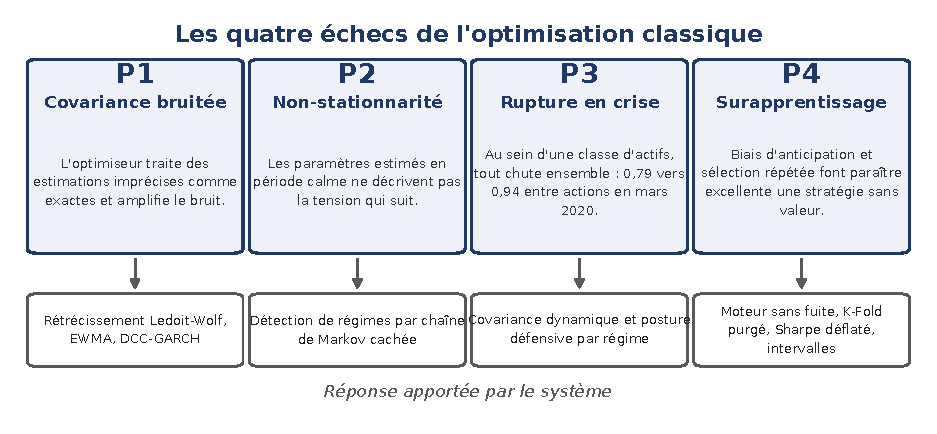
\includegraphics[width=\textwidth]{assets/figures/quatre_problemes.pdf}
  \caption[Les quatre problèmes P1--P4]{Les quatre échecs structurels de
  l'optimisation moyenne-variance classique, et la réponse apportée par le
  système développé. Chaque fonction du code source déclare, dans sa
  documentation, le ou les problèmes qu'elle adresse — une exigence de
  traçabilité vérifiée automatiquement par la suite de tests.}
  \label{fig:quatre-problemes}
\end{figure}

% -----------------------------------------------------------------------------
\subsection{P1 — L'estimation est bruitée}
% -----------------------------------------------------------------------------

Estimer une corrélation entre deux actifs à partir de quelques centaines
d'observations donne une valeur approximative. Avec neuf actifs, il faut estimer
36 corrélations et 9 volatilités simultanément, à partir du même historique
limité. Chacune porte son erreur.

Le problème n'est pas seulement que ces estimations soient imprécises : c'est que
l'optimiseur les traite comme exactes. S'il lit dans les données qu'un actif
possède une corrélation légèrement plus faible que les autres — un pur accident
d'échantillonnage — il conclut que cet actif est un excellent diversificateur et
lui attribue un poids considérable. L'optimiseur ne distingue pas le signal du
bruit ; il amplifie ce dernier.

\begin{remarquebox}
On résume souvent ce comportement en disant que l'optimisation moyenne-variance
est un \emph{maximiseur d'erreur d'estimation}. Ce n'est pas une critique de la
méthode, mais de son usage naïf : elle donne exactement ce qu'on lui demande, à
partir d'entrées dont on a négligé l'incertitude.
\end{remarquebox}

Le résultat pratique est un portefeuille concentré sur quelques positions, qui
paraît optimal sur l'historique utilisé pour le construire, et se comporte
médiocrement sur les données suivantes.

% -----------------------------------------------------------------------------
\subsection{P2 — Le monde ne reste pas immobile}
% -----------------------------------------------------------------------------

La théorie suppose implicitement que les rendements sont tirés d'une même loi de
probabilité, stable dans le temps. Les marchés ne se comportent pas ainsi. Ils
traversent des \emph{régimes} : des périodes calmes et haussières, des périodes
agitées et baissières, avec des transitions parfois brutales.

Concrètement, la volatilité se regroupe — les journées agitées se suivent — et
les corrélations elles-mêmes se déforment. Des paramètres estimés sur une période
calme décrivent mal la période de tension qui suit.

\begin{figure}[htbp]
  \centering
  
\includegraphics[width=\textwidth]{assets/figures/volatilite_regimes.pdf}
  \caption[Volatilité et régimes de marché]{Volatilité glissante du marché sur
  l'univers ETF du projet (2004--2026). Les périodes d'agitation sont
  manifestement groupées et non réparties uniformément~: c'est la
  non-stationnarité (P2), visible à l'œil nu. Les zones ombrées correspondent
  aux crises identifiées au chapitre~\ref{chap:resultats}.}
  \label{fig:volatilite}
\end{figure}

C'est précisément ce que le \emph{Machine Learning} peut apporter : plutôt que de
supposer un monde unique, on peut apprendre à reconnaître dans quel régime le
marché se trouve, et adapter la posture du portefeuille en conséquence.

% -----------------------------------------------------------------------------
\subsection{P3 — La diversification disparaît quand elle devient nécessaire}
% -----------------------------------------------------------------------------

C'est le plus contre-intuitif des quatre, et le plus coûteux.

En période normale, des actifs variés — actions marocaines, actions américaines,
or, obligations — évoluent avec une certaine indépendance. La diversification
fonctionne. Mais en période de crise, les investisseurs vendent
\emph{simultanément} tout ce qu'ils peuvent vendre pour se procurer des liquidités.
Les corrélations convergent alors vers~1 : tout baisse ensemble.

\begin{remarquebox}
Autrement dit : la protection que l'on a payée toute l'année en acceptant un
rendement moindre cesse d'agir exactement le jour où l'on en a besoin. Les
parapluies se referment quand la pluie commence.
\end{remarquebox}

Ce phénomène n'est pas théorique, et les données du projet permettent de le
mesurer. Elles apportent toutefois une nuance que la formulation usuelle omet, et
qui mérite d'être exposée telle quelle.

Si l'on calcule simplement la corrélation moyenne sur \emph{tous} les couples
d'actifs de l'univers, on obtient $0{,}24$ en période calme et $0{,}16$ en
crise~: la corrélation \emph{baisse}, ce qui contredit apparemment P3. Cette
moyenne est trompeuse, car elle agrège deux mouvements opposés. En les séparant
(figure~\ref{fig:correlations})~:

\begin{itemize}
  \item \textbf{entre actions} (SPY, QQQ, EEM), la corrélation passe de $0{,}79$
        en période calme à $0{,}85$ en crise, et culmine à $0{,}94$ lors du krach
        de mars~2020. P3 se vérifie pleinement~: à l'intérieur d'une même classe
        d'actifs, tout chute ensemble ;
  \item \textbf{entre actions et valeurs refuges} (or, obligations d'État
        longues), la corrélation, déjà quasi nulle en temps normal ($-0{,}04$),
        devient nettement négative en crise ($-0{,}18$)~: c'est la fuite vers la
        qualité, ces actifs montant lorsque les actions s'effondrent.
\end{itemize}

\begin{remarquebox}
La leçon est double, et elle oriente toute la suite du travail. D'une part P3 est
bien réel, mais il s'exprime \emph{au sein} d'une classe d'actifs. D'autre part
une diversification véritablement multi-classes conserve une partie de son
efficacité en crise — à condition que le portefeuille puisse effectivement se
déplacer vers les actifs qui se découplent. C'est exactement ce que fait
l'optimisation sous contrainte, et le chapitre~\ref{chap:resultats} montre
qu'elle protège en crise là où une répartition figée ne le fait pas.
\end{remarquebox}

\begin{figure}[htbp]
  \centering
  
\includegraphics[width=\textwidth]{assets/figures/correlations_crise.pdf}
  \caption[Rupture de la diversification en crise]{Corrélations glissantes
  (63~jours) sur l'univers ETF, décomposées par famille. En crise (zones
  ombrées), les actions se resserrent entre elles tandis que l'or et les
  obligations s'en détachent. Une moyenne calculée sur l'ensemble des couples
  masquerait ces deux effets en les compensant l'un par l'autre~— d'où la
  décomposition retenue ici.}
  \label{fig:correlations}
\end{figure}

% -----------------------------------------------------------------------------
\subsection{P4 — Se tromper soi-même : le surapprentissage}
% -----------------------------------------------------------------------------

Les trois premiers problèmes concernent les marchés. Le quatrième concerne
l'analyste, et c'est celui auquel ce projet a consacré le plus d'efforts.

Pour évaluer une stratégie, on la teste sur des données historiques : c'est le
\emph{backtest}. L'exercice est indispensable — et il est piégeux, pour deux
raisons distinctes.

\paragraph{Le biais d'anticipation (\emph{lookahead}).} Il consiste à utiliser,
au moment de décider, une information qui n'était pas encore disponible. Il prend
des formes très discrètes : normaliser des données sur l'historique complet avant
de découper le test, employer un cours de clôture non encore publié, ou choisir
un paramètre en observant le résultat final. Une stratégie affectée d'un biais
d'anticipation affiche des performances remarquables et ne les reproduit jamais
en conditions réelles.

\paragraph{Le surapprentissage par répétition.} Il est plus insidieux encore. En
essayant cinquante stratégies sur le même historique, on en trouvera
mécaniquement une qui paraît excellente — même si aucune n'a la moindre valeur.
C'est le hasard, et non la compétence, qui produit ce résultat. Publier la
meilleure sans mentionner les quarante-neuf autres revient à publier un mensonge
statistique, souvent commis de bonne foi.

\begin{remarquebox}
C'est le problème que l'encadrement du projet a désigné comme le critère de
correction le plus important : \emph{tout chemin par lequel une donnée future
pourrait influencer une décision passée constitue un échec automatique}. Le
chapitre~\ref{chap:architecture} montre comment cette exigence a été traduite en
une garantie structurelle plutôt qu'en une règle de discipline.
\end{remarquebox}

% =============================================================================
\section{Ce que le Machine Learning peut — et ne peut pas — apporter}
% =============================================================================

Il serait tentant de présenter le \emph{Machine Learning} comme la solution à ces
quatre problèmes. Ce serait inexact, et le présent rapport se garde de le faire.

\paragraph{Ce qu'il peut raisonnablement apporter.} Sur P1 et P2, l'apport est
tangible : des estimateurs de covariance plus élaborés qu'une simple moyenne
historique (rétrécissement de Ledoit-Wolf, moyennes exponentielles, modèles
GARCH) réduisent l'erreur d'estimation, et des modèles à variables latentes
(chaînes de Markov cachées) permettent de détecter un changement de régime sans
qu'on ait à le spécifier à l'avance. Sur P4, le \emph{Machine Learning} apporte
surtout sa \emph{méthodologie} d'évaluation — validation croisée adaptée aux
séries temporelles, correction du nombre d'essais, intervalles de confiance.

\paragraph{Ce qu'il ne peut pas apporter.} La prédiction fiable des rendements
futurs. C'est l'application que l'on attend spontanément, et c'est la plus
difficile : le rapport signal/bruit des rendements financiers est extrêmement
faible, et les marchés sont compétitifs par nature — toute régularité exploitable
tend à disparaître dès qu'elle est exploitée. Le chapitre~\ref{chap:resultats}
présente cinq tentatives indépendantes menées dans ce projet pour exploiter une
telle prédiction, et le résultat honnête auquel elles conduisent.

\begin{remarquebox}
Une distinction méthodologique importante, et vérifiée expérimentalement au
chapitre~\ref{chap:resultats} : améliorer la \emph{précision de prédiction} d'un
modèle n'améliore pas nécessairement la \emph{performance du portefeuille} qui en
découle. Ce sont deux objectifs différents, et le second n'est pas une
conséquence automatique du premier.
\end{remarquebox}

% =============================================================================
\section{Les contraintes réalistes de gestion}
% =============================================================================

Un dernier élément sépare l'exercice académique d'un prototype crédible : un gérant
professionnel n'est jamais libre de choisir n'importe quelle répartition. Il
opère sous contraintes, imposées par la réglementation, par son mandat ou par la
prudence.

\begin{itemize}
  \item \textbf{Pas de vente à découvert} — les poids sont positifs : on ne peut
        pas parier à la baisse sur un actif.
  \item \textbf{Un plafond par actif} — dans ce projet 25~\%, afin d'éviter les
        portefeuilles excessivement concentrés.
  \item \textbf{Des coûts de transaction} — chaque transaction se paie. Le projet
        retient 10 points de base sur les ETF internationaux et 30 sur les valeurs
        de la Bourse de Casablanca, moins liquides.
\end{itemize}

Le cahier des charges du client formule explicitement cette exigence de
« contraintes réalistes de gestion ». Elle a été traitée non comme une mesure
secondaire, mais comme une contrainte à part entière de l'optimiseur et du
simulateur. Nous verrons au chapitre~\ref{chap:resultats} que cette décision, prise
pour des raisons de réalisme métier, s'est révélée produire l'un des résultats les
plus marquants du projet.

% =============================================================================
\section{Problématique retenue}
% =============================================================================

L'ensemble de ce qui précède se résume en une problématique en trois volets, qui
sont ceux du présent rapport :

\begin{enumerate}
  \item \textbf{Construire} un système d'allocation de portefeuille exploitant le
        \emph{Machine Learning} pour répondre à P1, P2 et P3, sous des contraintes
        de gestion réalistes, et sur un univers combinant valeurs de la Bourse de
        Casablanca et ETF internationaux.
  \item \textbf{Évaluer} ce système avec une rigueur suffisante pour que P4 ne
        puisse pas invalider les conclusions : absence de biais d'anticipation
        garantie par construction, données de test jamais utilisées pour le choix
        des paramètres, et intervalles de confiance sur chaque chiffre publié.
  \item \textbf{Rapporter} honnêtement ce que le système apporte et ce qu'il
        n'apporte pas — un résultat négatif correctement établi ayant, dans ce
        domaine, davantage de valeur qu'un résultat positif invérifiable.
\end{enumerate}

% =============================================================================
\section{État de l'art}
% =============================================================================

Les travaux sur lesquels le projet s'appuie sont les suivants.

\paragraph{Markowitz (1952).} \emph{Portfolio Selection} est le texte fondateur qui
introduit le cadre moyenne-variance et la frontière efficiente. Il constitue la
référence par rapport à laquelle tout le reste se compare.

\paragraph{DeMiguel et al. (2009).} Dans \emph{Optimal Versus Naive
Diversification}, les auteurs établissent un résultat célèbre et dérangeant : sur de nombreux jeux de
données, le portefeuille équipondéré — répartir également, sans rien estimer —
fait aussi bien, voire mieux, que les portefeuilles optimisés, une fois les coûts
pris en compte. Précisément parce qu'il n'estime rien, il ne peut pas
surapprendre le bruit. Ce portefeuille sert dans ce projet de \emph{haie
d'honnêteté}~: toute méthode sophistiquée doit d'abord démontrer qu'elle le
dépasse.

\paragraph{Ledoit et Wolf (2004), \emph{shrinkage} de covariance.} Réponse
statistique directe à P1 : rapprocher la matrice de covariance empirique d'une
cible structurée, avec une intensité estimée sur les données elles-mêmes.

\paragraph{Engle (2002), \emph{Dynamic Conditional Correlation}.} Réponse à P2 au
niveau de l'estimation : un modèle où volatilités et corrélations évoluent dans le
temps plutôt que d'être supposées constantes.

\paragraph{Jagannathan et Ma (2003), \emph{Risk Reduction in Large Portfolios}.}
Résultat théorique important pour ce projet : imposer une contrainte de poids
active équivaut mathématiquement à opérer un rétrécissement de la matrice de
covariance. Autrement dit, une contrainte de gestion réaliste effectue
implicitement le travail de régularisation que l'on attend d'une méthode
sophistiquée. Le chapitre~\ref{chap:resultats} reproduit ce résultat sur les
données du projet.

\paragraph{López de Prado (2018), \emph{Advances in Financial Machine Learning}.}
Ouvrage de référence sur P4. Deux outils en sont directement repris : la
\emph{purge} et \emph{embargo} — qui retirent du jeu d'entraînement les
observations temporellement voisines du jeu de validation, appliqués ici dans un
découpage strictement antérieur plutôt qu'en blocs (chapitre~\ref{chap:modelisation})
— et le \emph{Deflated Sharpe Ratio} de Bailey et López de Prado (2014), qui corrige un ratio de Sharpe observé
du nombre de stratégies essayées pour l'obtenir.

% =============================================================================
\section*{Synthèse du chapitre}
\addcontentsline{toc}{section}{Synthèse du chapitre}

L'allocation de portefeuille consiste à répartir un capital entre plusieurs
actifs de manière à maximiser le rendement tout en maîtrisant le risque. La
théorie classique de Markowitz formalise ce compromis, mais suppose connus des
paramètres qui doivent en réalité être estimés à partir d'un historique limité.
Il en découle quatre difficultés : l'amplification du bruit d'estimation (P1), la
non-stationnarité des marchés (P2), l'effondrement de la diversification en
période de crise (P3), et le risque que l'analyste se trompe lui-même en
évaluant sa propre stratégie (P4).

Le \emph{Machine Learning} offre des réponses crédibles à P1 et P2, une réponse
partielle à P3, et surtout — c'est le point le moins attendu — un appareil
méthodologique pour traiter P4. Il n'offre pas, en revanche, de prédiction fiable
des rendements futurs.

Le chapitre suivant décrit l'architecture du système construit pour répondre à
cette problématique, en commençant par l'infrastructure de données sur laquelle
tout le reste repose.
